\appendix
\section{Source code}
\UseRawInputEncoding
Code for Shor's algorithm for integers composed of Fermat's prime: $shorforfermat.py$
\lstinputlisting[language=Python]{shorforfermat.py}


Code for creating graph \ref{fig: MEF periodic output graph}: $forMEFgraph.py$ 
\lstinputlisting[language=Python]{forMEFgraph.py}

Code to plot  the  graph   showing the complexity  of  Shor's algorithm  and  number  field  sieve: $Complexity_shor_vs_sieve.py$
\lstinputlisting[language=Python]{Complexity_shor_vs_sieve.py}


\section{Numerical implementation}
We discuss two approaches of numerical implementation: an approach using number theory background and an approach involving direct use of Shor's algorithm.
\subsection{Number theory approach}
Consider an integer to be factored: $I = 15$
\\
\\ First we consider a random number $z=2$
\\ $GCD(15,2)=1$, 15 and 2 are co-prime
\\ $f(x) = 2^x$ mod 15 for $x\in \mathbf{N}$ gives
\\
\begin{table}[ht]
    \centering
\begin{tabular}{|c|c|c|c|c|c|c|c|c|c|c|c|c|c|c|}
\hline
f(0) & f(1) & f(2) & f(3) & f(4) & f(5) & f(6) & f(7) & f(8) & f(9) & f(10) & f(11) & f(12) & f(13) & f(14) \\ \hline
1  &2     & 4    & 8    & 1      &2  & 4    & 8    & 1   &2   & 4    & 8    & 1  &2   & 4       \\ \hline
\end{tabular}
 \caption{Example of implementation:$f(x) =2^x$ mod 15}
 \label{tab: Example of implementation:$f(x) =2^x$ mod 15}
\end{table}

The period of function $f(x)$ is 4.

Now, according to \ref{th:factors_GCD_pm}, the factors are $GCD(2^\frac{4}{2}+ 1, 15) = 5 $ and $GCD(2^\frac{4}{2}- 1,15)=3$

\subsection{Shor's algorithm approach}
In this approach, we would use apply Shor's algorithm numerically on an integer. This method involves working with probabilities and histogram. We discuss the application of Shor's algorithm, on two different set of examples:
\subsubsection{Example I: $m=\tilde{m}$}
Let a number to be factored be $I= 15$
\\ Using the inequality $I^2 \leq 2^n = N \leq 2I^2$, we get, $N=256$
Also, we get $r= \lfloor 2logI \rfloor +1 \simeq 4$
\\ Hence, the initialized register is $\psi_1 = \ket{0}^8\ket{0}^4$

Upon application of Hadamard gates on 1st register, we get
$$\psi_2 = \frac{1}{\sqrt{256}} \sum_{x=0}^{255} \ket{x}^8\ket{0}^4 = \frac{1}{\sqrt{256}} (\ket{0}\ket{0} + \ket{1}\ket{0},\dots , \ket{255}\ket{0}) $$

The modular exponential function $f(x)= z^x$ mod $I$ where $z$ is a randomly selected integer less than I.
\\Let the randomly selected integer $z=2$
\\So, $f(x) = 2^x$ mod $15 $

First few terms of $f(x)$ are:
{\scriptsize $$\begin{matrix}
      1  &   2  &   4  &   8  &   1  &   2  &   4  &   8 \\
  1  &   2  &   4  &   8  &   1  &   2  &   4  &   8 \\
  1  &   2  &   4  &   8  &   1  &   2  &   4  &   8 \\
  1  &   2  &   4  &   8  &   1  &   2  &   4  &   8 \\
  1  &   2  &   4  &   8  &   1  &   2  &   4  &   8 \\
  1  &   2  &   4  &   8  &   1  &   2  &   4  &   8 \\
  1  &   2  &   4  &   8  &   1  &   2  &   4  &   8 \\
  1  &   2  &   4  &   8  &   1  &   2  &   4  &   8 \\
  
\end{matrix}$$}
\\We can clearly see that it has the order, $a=4$ and frequency $m = \frac{N}{a}= 64$

Now applying $f(x)$ on second register,
 $$\psi_3 = \frac{1}{\sqrt{256}} \sum_{x=0}^{255} \ket{x}^8\ket{f(x)}^4 =  \frac{1}{\sqrt{255}}  \sum_{j=0}^{63} \sum_{x=0}^{4} \ket{x +4j} \ket{f(x)}$$
 
Upon conceptual measurement, let the second register collapse to $f(5)$. Then, the first register collapses correspondingly to following state:
$$\psi_4 = \frac{1}{\sqrt{64}} \sum_{j=0}^{63} \ket{3+6j} \ket{2^3 mod 15} $$
$$\psi_4 = \frac{1}{\sqrt{64}} ( \ket{3} + \ket{7} +\ket{11}+ \dots + \ket{255} )$$
Upon application of QFT on first register, we get:
$$\psi_5 = \sqrt{\frac{m}{N}} \sum_{c=0}^{3} e^{\frac{2i\pi  64c}{m}} \ket{64c} $$
$$= \frac{1}{2} (\ket{0} + \ket{64} + \ket{128} + \ket{192} )$$

Upon measurement of first register, we obtain a set$\{y_c\} = \{0,64,128,192\}$ with higher probabilities than others.

The histogram represents classical fast Fourier transform on $f(x)$ which represents the similar output as calculated numerically.
\begin{figure}[H]
    \centering
    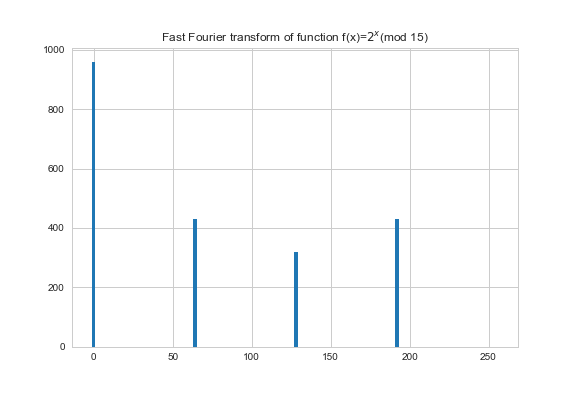
\includegraphics[scale=0.45]{figures/fft_on_2^xmod15.png} 
    \caption{Output after applying \acrshort{FFT} on $f(x)$}
    \label{fig: fft_on_2^xmod15_2}
\end{figure}

Now,we take the GCD of the possible states: $GCD(64, 128, 192) = 64$
The period/order is $$a=\frac{N}{m}= \frac{256}{64}= 4$$.
S, the factors are $GCD(2^{\frac{a}{2}} \pm 1, 15)$ = $GCD(5,15)$ and $GCD(3,15)$ = 5 and 3.

\subsubsection{Example II: $m\neq \tilde{m}$}
For this example, we take a different number to be a factor, $I=21$. Similarly as in example I, we get $N=512, n=9$ and $r=4$.

Hence the initialized register be $\psi_1 = \ket{0}^9\ket{0}^4$

Upon applying Hadamard on 1at register, we get
$$\psi_2 = \frac{1}{\sqrt{512}} \sum_{x=0}^{511} \ket{x}^9\ket{0}^4 = \frac{1}{\sqrt{512}} (\ket{0}\ket{0} + \ket{1}\ket{0},\cdots , \ket{511}\ket{0}) $$

Let $z=2$ be randomly selected integer for the modular exponential function $f(x)= z^x$ mod $I$.
So, $f(x) = 2^x$ mod $21 $

First few terms of $f(x)$ are 
{\scriptsize $$\begin{matrix}
     1  &   2  &   4  &   8  &  16  &  11  &   1  &   2 \\
  4  &   8  &  16  &  11  &   1  &   2  &   4  &   8 \\
  16  &  11  &   1  &   2  &   4  &   8  &  16  &  11 \\
  1  &   2  &   4  &   8  &  16  &  11  &   1  &   2 
\end{matrix}$$}
\begin{figure}[H]
    \centering
    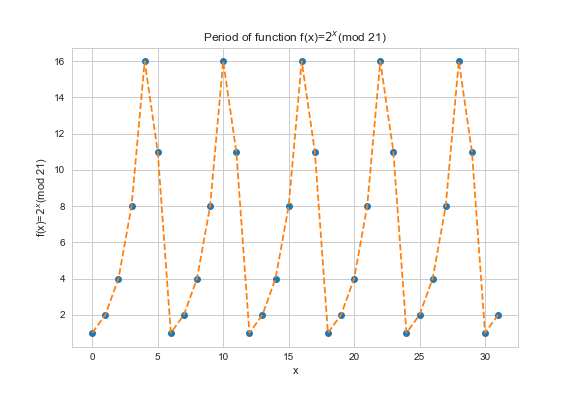
\includegraphics[scale=0.4]{figures/periodicfunction(2,21).png} 
    % \caption{}
    \label{fig: periodicfunction(2,21)}
\end{figure}
From the figure(\ref{fig: periodicfunction(2,21)} and terms, we can clearly see it has the order, $a=6$. The task is to determine the order computationally.

Now applying $f(x)$ on second register,
 $$\psi_3 = \frac{1}{\sqrt{512}} \sum_{x=0}^{511} \ket{x}^9\ket{f(x)}^4 =  \frac{1}{\sqrt{64}} \sum_{j=0}^{\tilde{m}} \sum_{x=0}^{6} \ket{x +6j} \ket{f(x)}$$ where $\tilde{m}$ is the frequency of $f(x)$.
 
Since at $x=255$ the function $f(x)$ does not complete the full cycle,
$$ \tilde{m} = \begin {cases}
    m = 86 &\text {for f(x)=\{1,2\}} \\
    m = 85 &\text {for f(x)=\{4,8,15,11\}}
    \end{cases}  $$
Upon conceptual measurement, let the second register collapse to $f(5)$. Then, the first register collapses correspondingly to following state:
$$\psi_4 = \frac{1}{\sqrt{85}} \sum_{j=0}^{85} \ket{5+6j} \ket{2^5 \:mod\: 21} $$
$$\psi_4 = \frac{1}{\sqrt{85}} ( \ket{5} + \ket{11} +\ket{17}+ \dots + \ket{510} )$$
Upon application of QFT on first register, we get:
$$\psi_5 = \frac{1}{\sqrt{512*85}} \sum_{j=0}^{512} \sum_{j=0}^{85} e^{\frac{2i\pi (5+6j)y }{256}} \ket{y} $$
According to the theory, upon measuring the 1st register, we get a set of outputs $y_c\rfloor_{c=0}^{5}$ with higher probabilities than others. The set $y_c\rfloor_{c=0}^{5}$ satisfies:
$$a y_c \in [cN-a/2, cN+a/2]$$
$$6 y_c \in [cN-6/2, cN+6/2]$$
By computation, the $y_c's$ are $\{0,85, 171, 256, 341, 427\}$.

The histogram represents classical fast Fourier transform on $f(x)$ which represents the similar output as calculated numerically.
\begin{figure}[H]
    \centering
    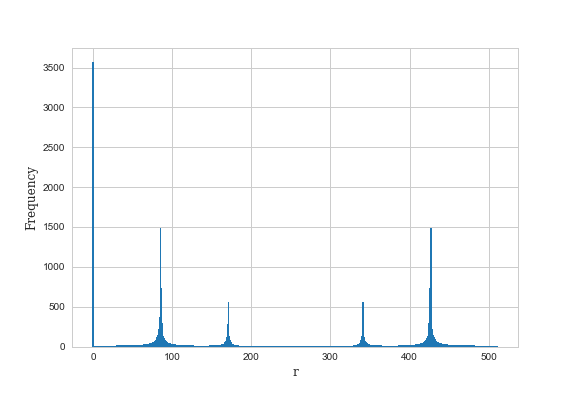
\includegraphics[scale=0.45]{figures/fft_on_2^xmod21.png} 
    \caption{Output after applying \acrshort{FFT} on $f(x)$}
    \label{fig: fft_on_2^xmod21}
\end{figure}
Now we use $y_c's$ to compute period,$a$.
We apply Continued fraction algorithm on a set $\frac{y_c}{N}\rfloor_{c=0}^{5} = \frac{y_c}{512}\rfloor_{c=0}^{5}$ . And from 5.3.7: Claim 2,Continued fraction Algorithm on $\frac{y_c}{N}$ with error $\frac{a}{2I^2}$ outputs unique $\frac{c}{a}$. For example,
\\ The convergents of  $\frac{85}{512}$ are $\{\frac{1}{6}, \frac{42}{253}\}$
\\ Then $\abs{\frac{85}{512} -\frac{1}{6}}<\frac{1}{2*{21}^2}$
but $\abs{\frac{85}{512} -\frac{42}{253}}>\frac{1}{2*{21}^2}$.

So, $\frac{85}{512}$ converges to $\frac{1}{6}$. Similarly, all elements in set $\{y_c\}$converges to a set $\{\frac{1}{6},\frac{1}{3},\frac{1}{2},\frac{2}{3}, \frac{5}{6}, 1$.
\}
We know, $\{\frac{y_c}{N}\}_{c=0}^5$ converges to $\{\frac{c}{a}\}_{c=0}^5$. Hence comparing the above set, the period is $a=6$.

Similarly as above, the factors are obtained from $GCD(2^{\frac{6}{2}} \pm 1, 21)$= $GCD(7,21)$ and $GCD(9,21)$. The factors are 7 and 3.

